% Partial Credit System Diagram
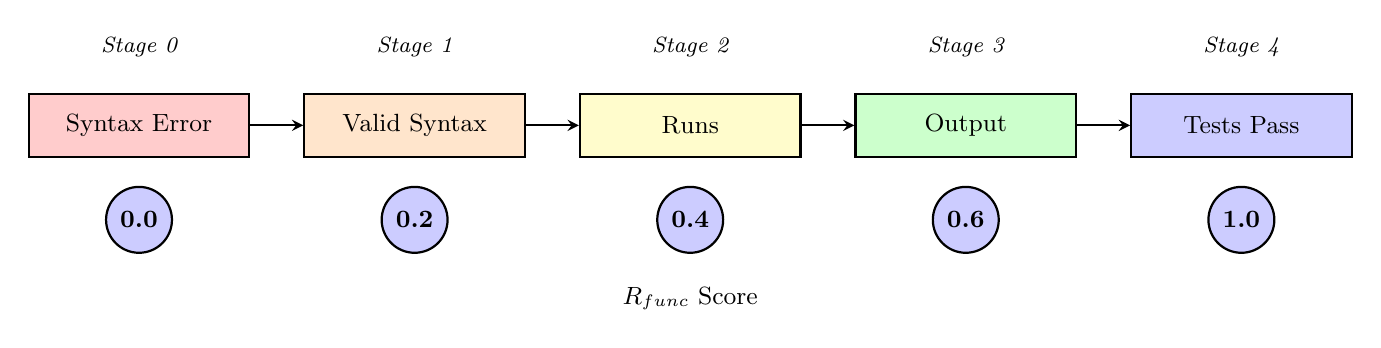
\begin{tikzpicture}[
    box/.style={rectangle, draw=black, thick, minimum width=2.8cm, minimum height=0.8cm, align=center, font=\small},
    score/.style={circle, draw=black, thick, fill=blue!20, minimum size=0.8cm, font=\small\bfseries},
    arrow/.style={->, thick, >=stealth}
]

% Boxes (stages)
\node[box, fill=red!20] (s0) at (0,0) {Syntax Error};
\node[box, fill=orange!20] (s1) at (3.5,0) {Valid Syntax};
\node[box, fill=yellow!20] (s2) at (7,0) {Runs};
\node[box, fill=green!20] (s3) at (10.5,0) {Output};
\node[box, fill=blue!20] (s4) at (14,0) {Tests Pass};

% Scores below
\node[score] at (0,-1.2) {0.0};
\node[score] at (3.5,-1.2) {0.2};
\node[score] at (7,-1.2) {0.4};
\node[score] at (10.5,-1.2) {0.6};
\node[score] at (14,-1.2) {1.0};

% Arrows
\draw[arrow] (s0) -- (s1);
\draw[arrow] (s1) -- (s2);
\draw[arrow] (s2) -- (s3);
\draw[arrow] (s3) -- (s4);

% Labels
\node[above of=s0, node distance=1cm, font=\footnotesize\itshape] {Stage 0};
\node[above of=s1, node distance=1cm, font=\footnotesize\itshape] {Stage 1};
\node[above of=s2, node distance=1cm, font=\footnotesize\itshape] {Stage 2};
\node[above of=s3, node distance=1cm, font=\footnotesize\itshape] {Stage 3};
\node[above of=s4, node distance=1cm, font=\footnotesize\itshape] {Stage 4};

% Title
\node[font=\small] at (7,-2.2) {$R_{func}$ Score};

\end{tikzpicture}
